\setcounter{chapter}{3}
\setchapterabstract{Market power, a firm's ability to raise prices above competitive levels, is crucial in antitrust analysis. It's a prerequisite for investigating anticompetitive practices under various legal frameworks. This chapter explores the definition, measurement, and constraints of market power. By understanding market power, antitrust authorities can effectively identify and address harmful practices that impact consumer welfare.}
\chapter{Market Definition and Market Power}
\vspace{-1.5cm}

{\chaptoc\noindent\begin{minipage}[inner sep=0,outer sep=0]{0.9\linewidth}\section{Market Power}\end{minipage}}

    \begin{figure}[h]
        \centering
        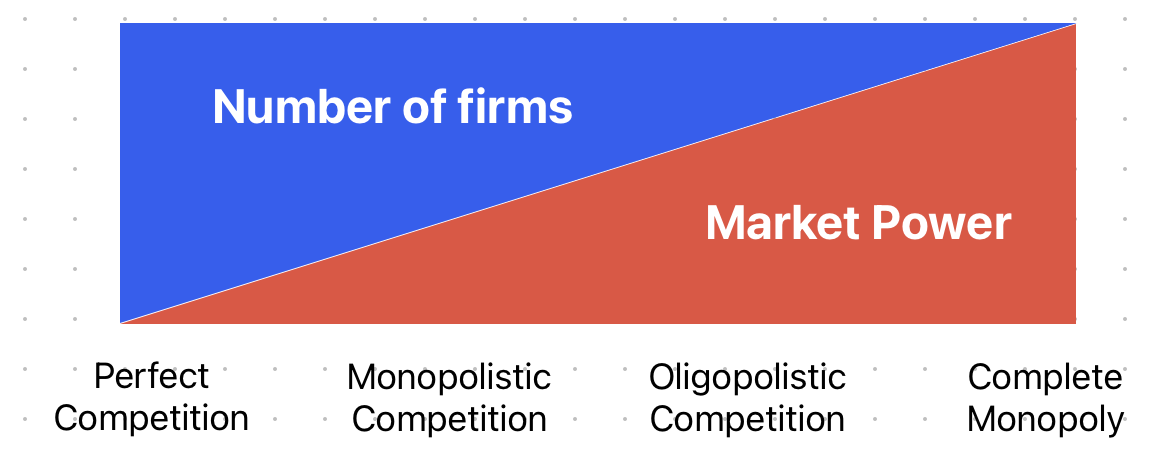
\includegraphics[width=0.5\linewidth]{market_power.png}
    \end{figure}

    The definition and measurement of market power is key in antitrust because firms can negatively affect CS only when they hold “some” degree of Market Power (MP is needed to cause a significant deviation from the natural development path of the market).
    \begin{itemize}
        \item In \textbf{Art. 102 cases}, MP is fundamental to establish whether the structural element is met (Art. 102: a high level of market power, labeled as “dominant position”, is a prerequisite for the application of the prohibition);
        \item \textbf{Art. 101}. In cases other than by object restrictions (cartels), MP is needed to establish whether the arrangement is anticompetitive (de minimis non curat praetor);
        \item \textbf{Reg. 139/2004}: appraisal of combined MP to establish whether a merger is anticompetitive. The (empty) test is that of a significant lessening of competition. The EU Commission’s Guidelines on horizontal mergers fill up this test by stating that a merger is incompatible when it creates or reinforces a dominant position or a very concentrated market structure in which anticompetitive non-coordinated or coordinated effects are likely.
    \end{itemize}

        \subsubsection{How can we define market power (MP)?}

            \begin{quote}
                 "Market power comes from the ability to cut back the market's total output and so raise price”
            \end{quote}
            Ball Memorial Hospital, Inc. v. Mutual Hospital Insurance, Inc., 784 F.2d 1325, 1335 (1986).

            \Definition{“The ability of a firm (or group of firms) to raise and maintain price above the level that would prevail under competition is referred to as market or monopoly power. The exercise of market power leads to reduced output and loss of economic welfare”}{OECD Definition of Market Power}

            MP does not refer only to price and output: the ability to… limiting consumer choice, product quality, or reducing innovation, signals that a certain firms enjoys market power.\sn{\Note{In this set of slides we will focus on market/ monopoly power, but you may also think to monopsony power}}

            If market power is the ability of a firm to profitably raise the market price of a good or service over its marginal cost thus:
            \begin{itemize}
                \item In perfectly competitive markets, market participants entail no market power (they are “\textbf{price taker}”).
                \item On the contrary, when a firm enjoys MP, it can raise prices without losing any customers to competitors. Market participants that have MP are therefore sometimes referred to as "\textbf{price makers}" or "\textbf{price setters}” .
            \end{itemize}
            Significant MP occurs when prices exceed marginal cost and long term average cost, so the firm makes (extra) profits.

    \subsection{The technical notion and its problems: From Market Power to Relevant Markets}

        \Definition{The Lerner Index (LI) quantifies MP with the following equation:
        \begin{equation}
            \frac{P-MC}{P} = \frac{Q\delta(P)}{P\delta(Q)} = \begin{cases}
                0 & \text{ with perfect competition} \\
                1 & \text{ with monopoly}
            \end{cases}
        \end{equation}}{Lerner Index}

        Antitrust enforcers usually do not apply LI\sn{\Note{Essentially, the index measures the percentage markup that a firm is able to charge over its marginal cost. It ranges from a low value of 0 to a high of 1. The higher the value of the LI, the more the firm is able to charge over its marginal cost, hence the greater its monopoly power. The LI provides a concise measure of monopoly power.}}, because marginal costs are very difficult to measure… especially in courtrooms. Alternative tools and methodologies bump into similar problems. Thus, AA use other tools to appreciate market power, starting to a proxy: Market shares (MS). After all, there is a positive correlation between MP and MS: it can be shown that the LI is positively correlated with market shares. If \(MS \uparrow \rightarrow LI \uparrow\).

        \Remark{
        However to calculate MS, we need to define the \textbf{relevant market}.
        }

\section{Relevant Market}

        \subsubsection{Relevant Markets as the first step of the competitive analysis}

            To measure MP (and MS) we need to identify the market where a firm interacts with its upstream suppliers, horizontal competitors, and downstream users/costumers. Thus, identification of the relevant market should logically come first\sn{\Remark{
            In some instances, the definition of relevant markets is less important or not necessary (cartels are prohibited by object; no need to determine their effect).
            }}, and MP appraisal should follow (even if this has not always proved true, especially in the context of abuses of dominance). The exercise should be carefully done: the larger is the “area” of the relevant market, the lower the possibility of finding MP (but also the opposite may be dangerous, especially when dealing with local markets).

            \Example{
                \begin{tabular}{|c|c|c|c|}
                    \hline
                     & \textbf{Colas} & \textbf{Carb. Soda beverages} & \textbf{All beverages} \\
                     \hline
                    \textbf{Coca Cola} & 95\% & 70\% & 2\% \\
                    \hline
                \end{tabular}
            \hspace{3cm}
            Can Coca Cola defend itself by saying that“all beverages have as basic function to quench the consumer's thirst”, so that tap water, colas and gin belong to the same market?
            }

        \subsubsection{History}

            The relevant market was first-ever used in 1948 in the U.S. Supreme Court case United States v. Columbia Steel Co., in response to the need to determine the geographical boundaries of post- merger competitive effects. And guess who was the parent company of Columbia Steel since 1930 ? US Steel

    \subsection{Relevant Markets: the EC Commission’s Definition (new 2024 Guidelines)}

        Market definition is a tool that the Commission uses to identify and define the boundaries of competition between undertakings. The main purpose of market definition is to identify in a systematic way the effective and immediate competitive constraints faced by the undertakings involved when they offer particular products in a particular area. Market definition leads to the identification of the relevant competitors of the undertaking(s) involved when they offer those products, as well as the relevant customers. Only products that exert effective and immediate competitive constraints within the relevant time frame form part of the same relevant market as those of the undertaking(s) involved, while other less effective, or merely potential, constraints are considered as part of the competitive assessment

        \subsubsection{The Notion of Relevant Market (pittfalls)}

            When it comes to market definition, there is no certainty, no black or white solution:
            \begin{enumerate}
                \item[a.] the parties have different approaches, and sometimes conflicting interests
                \item[b.] markets change according to many factors, such as time, preferences, technology, innovation. Furthermore, they may change according to the specific infringement under investigation.
            \end{enumerate}

            \noindent
            In addition, often it happens that data are:
            \begin{enumerate}
                \item Not available;
                \item Not reliable, or too old, or incomplete;
                \item Open to different/conflicting interpretations.
            \end{enumerate}

        \subsubsection{The Notion of Relevant Market}

            AAs usually distinguish between:
    
            \Definition{Product market, which includes all those products and/or services that can be regarded as substitutable. AAs assess interchangeability looking at “substitution of demand” and (sometimes) “substitution of supply” ;}{Product market}
    
            \Definition{Geographical market, which comprises the area where the firms in question act under sufficiently homogeneous conditions;}{Geographical market}
    
            \Definition{Temporal market, for seasonal products of services (e.g.bananas vs. seasonal fruit in the UK and Ireland in the 60’ ; peak/off peak services, hotels vs other accommodations}{Temporal market}

        \subsubsection{Timing of the Analysis}

            \begin{itemize}
                \item \textbf{For agreements + abuses of a dominant position} the analysis is backward looking. The task is to ascertain weather a certain conduct already conceived (and usually put into effect) caused or could have led to adverse effects in terms of CS. Thus, the exercise of determining market power is influenced by the particular moment at which the evaluation takes place (ex post analysis of markets and market power).
                \item \textbf{For mergers} the analysis of relevant market is forward looking. The question to be answered is how the relevant market will be shaped once the merger will be completed. Thus, you also have to consider the likely reaction of actual and potential competitors and the possible evolution of markets in the short/medium run (ex ante analysis of markets and market power).
            \end{itemize}

\section{Product Market}

        \subsubsection{Demand Substitution}

            AA need to understand:
            \begin{itemize}
                \item \textbf{whether} consumers will abandon the product of the firm under scrutiny when it will increase its price above the market price
                \item \textbf{how many} consumers will abandon the product of the firm under scrutiny when it will increase its price above the market price
            \end{itemize}

            To accomplish this goal, AA need to identify the goods/services that can substitute the products of the firm under scrutiny. In other words, the products to which consumers may switch, when the firm under investigation increases its price above the competitive price.

        \subsubsection{Assessing Demand Substitutability}

            \noindent
            To assess demand substitutability, we look at many factors, such as:
            \begin{enumerate}
                \item consumers’ tastes and preferences;
                \item products' features;
                \item the manners in which products are actually used;
                \item the manners in which they are distributed;
                \item products’ prices;
            \end{enumerate}

            AAs use several sources of information regarding the past functioning of the market, such as data and analyses submitted by the undertakings involved in the case; consumers’ surveys and competitors’ opinions; statistical \& econometric market studies; etc…

        \subsubsection{SSNIP Test}

            Furthermore, they can use a quantitative tool, such as the so-called SSNIP (Small but Significant, and Non-Transitory Increase in Price) test based upon cross-elasticity of demand.
            The question to be addressed is whether the parties' customers would switch to readily available substitutes in response to a hypothetical small (in the range 5-10\%), but permanent relative price increase in the products being considered.

            Methodology:
            \begin{itemize}
                \item Start with smallest possible market and find if a 5-10\% price increase is profitable; If enough costumers shift to another available product, the price increase is not profitable. This means that the firm does not have sufficient market power to raise prices. In this circumstance, the next closest substitute is added to the relevant market and the same test repeated.
                \item Process continues until the point is reached where a hypothetical monopolist could profitably impose a 5\% price increase. To know more, see this \href{https://www.youtube.com/watch?v=5VE6FaCILaU}{video by David Evans}.
            \end{itemize}

            \Example{
            \textbf{Speed cars:}
            Let’s start considering the Ferrari 812 “superfast” (F) as the hypothetical monopolistic product.
            \begin{itemize}
                \item[Step 1:] if the price of a F goes up by 5-10\%, is there any kind of substitution with other luxury speed cars?, i.e.: do consumers start buying other cars, like Porsche (P), Lamborghini (L) Maserati (M)?
                \begin{enumerate}
                    \item \textbf{No}: the product market corresponds to Ferrari cars.
                    \item \textbf{Yes}, than F, P, L, and M belong to the same product market. In that event, you must go on with the SNIPP test.
                \end{enumerate}
                \item[Step 2:] if the price of F, P, L and M goes up by 5-10\%, do consumers start buying sports cars like a Ford Mustang? Again, if the answer is positive, it means that luxury speed cars and sports cars belong to the same product market; if the answer is negative, sports cars do not belong to the luxury speed cars market.
            \end{itemize}
            }

        \subsubsection{Role of tastes and preferences}

            “There are three different ways of treating milk: pasteurization (for fresh milk), UHT, and sterilization (for aseptically packed milk)… whilst each type of milk may technically be an adequate or acceptable substitute for the other types, in that it is a liquid with certain nutritional properties, consumers do not regard them as perfectly interchangeable, because of different tastes and preservation qualities. Therefore, we have three different relevant markets: that for fresh milk, that for UHT and that for sterilized milk”\sn{\Note{Does that distinction still hold nowadays? Tech evolution may influence the shape of relevant markets}} EC Commission 26 July 1988, IV/31.043 - Tetra Pak I.

        \subsubsection{Role of products’ features and uses}

            \textbf{Flat Glass:} “flat glass is not interchangeable [...] with other products in respect of the various applications for which it is intended. Leaving aside use for greenhouses and verandas, in respect of which flat glass is in competition with plastic, unless there is a particular need to avoid heat dispersion, there are no competing products for the other uses of flat glass. In the case of automotive glass, building glass, mirrors, reflecting glass, insulating glass, laminated glass and armoured glass, flat glass cannot be replaced by other products.\sn{\Note{Flat glass must consequently be considered to be a specific market, except in the case of [greenhouses and verandas]” – see COMMISSION, 7 December 1988, Flat Glass.}}

        \subsubsection{Supply Substitution (sleeping or latent competitors)}

            Supply substitution can be employed to reinforce the conclusions reached by analysing the demand substitution:

            \Example{
            Steel mills produce and use oxygen for their blast furnaces and thus produce steel , but this oxygen is then wasted , dispersed into the atmosphere . If the price of oxygen( used , for example , for lung diseases ) were to rise considerably, steel mills might decide to enter the market and compete with existing medical oxygen producers. Two options: either we consider sleeping competitors as part of the relevant market; or we consider their possible role at a later stage.
            }

        \subsubsection{The European Commission's approach}

            \Definition{Supply substitution can also be relevant for the definition of the relevant market in some cases, namely when it is as effective and immediate as demand substitution and when it leads to similar competitive conditions across the products concerned. In the Commission’s experience, supply substitution is only relevant for market definition in specific cases}{2024: EU Commission Guidelines on relevant markets, paragraph 23(b)}

            Otherwise, supply side is considered, together with potential competition, at a later stage, i.e. when analysing the competitive constraints to market power\sn{\Note{Do you think that it really changes the outcome of the analysis?}}.

            
\newpage
\section{Relevant Geographic Market}

        \subsubsection{Geographic Market definition in Theory (SNIPP again)}

            Again, the theoretical method to define geographic market relies on the SNIPP test: we start by delineating the geographic market to be a region such that a hypothetical monopolist (“M” is the only producer of the relevant product in that region) would profitably impose at least a "small but significant and nontransitory" increase in price.
            Assume that buyers can respond to a price increase on goods produced within the identified region by shifting to goods produced outside the region. If those locations of production outside the region are sufficiently attractive at their existing terms of sale, an attempt by “M” to raise the price would result in a reduction in M’s sales large enough that the price increase would not be profitable. This means that the initially identified geographic area is too narrow.

        \subsubsection{Goal}

            Antitrust enforcers need to understand if geography limits some customers’ willingness or ability to substitute to some products, or some suppliers’ willingness or ability to serve some customers.

        \subsubsection{Task}

            In order to accomplish this goal, antitrust enforcers need to focus on many and diverse elements, such as:
            \begin{enumerate}
                \item Supplier and customer locations
                \item Consumers’ tastes and conduct
                    \begin{itemize}
                        \item languages (as in the cases of pharmaceutical products and toys, books, TV broadcasting, newspapers, movies, magazines);
                        \item culture and lifestyle (as in the case of morning goods);
                    \end{itemize}
                \item Market features and constraints.
                    \begin{itemize}
                        \item Trade flows and pattern of shipments (as in the case of raw materials; gas, etc.);
                        \item Transportation costs (mineral water) and the speed of Deterioration of certain goods.
                    \end{itemize}
                \item Barriers to entry
            \end{enumerate}

\newpage
        \subsubsection{Examples: how far can consumers go?}

            \Example{
            \textbf{The market for concerts}
            \begin{itemize}
                \item The distance that a theatre fan will travel to attend to a drama cannot easily be rationalised on the basis of transportation costs. See Houser v. Fox Theatres Mgmt. Corp., 845 F.2d 1225, 1230 \& n, 10 (3d Cit. 1988), holding that relevant market is a single municipality because most (but not all) theatre-goers were local and limited their patronage to local theatres.
                \item But would you reach the same conclusion for hip-hop, Pop, Rap music ? 
                \item My daughter asked me: what happens if your students don’t know know Lauryn or at least the Fugees ?
                \item I appeal to the fifth amendment and to the right to stay silent.
            \end{itemize}
            }

            \Example{
            \textbf{GeoMarkets for medical services}
            \begin{itemize}
                \item Differently, for essential medical services, customers may be willing to travel a considerable distance. 
                \item See Morgan, Strand, Wheeler \ Biggs v, Radiology, Ltd., (9th Cir.1991), refusing to limit the market for radiology services to a single city; 
                \item See United States v. Mercy Health Services, (N.D.Iowa 1995), holding that the relevant geographic market was of at least a 70-mile radius because some people in the defendant hospital’s town (Dubuque, Iowa) travelled to a hospital 70 miles away (in Cedar Rapids, Iowa) for cosmetic surgery.
                \item But query: do people having heart attacks, or highway accident victims also would travel 70 miles when there is a hospital in their home town? See, e.g., Brader v. Allegheny General Hospital, 64 Fad 869 (3d Cir. 1995), defining a narrower local geographic market for vascular and traumatic care services.
            \end{itemize}
            } 

        \subsubsection{Let’s look to some more complex cases}

            \begin{enumerate}
                \item Which is the Geographic Market for Motorways’ Oil Service Stations? (how many kilometers can you cover when you are low on gasoline?) And outside the Motorways ? (suppose that you are examining the potential adverse effect of the merger of two small service stations near Bocconi University)
                \item Which is the Geographic Market for banking products ? Let’s go back to 1998 (no online banking): Deposits/loans (credits) ? Is technological change contributing to shape different geographic/product markets ?
                \item Market Asymmetries. New York vs. Jersey City
            \end{enumerate}

\section{Market Power}

    Market power is studied and assessed on the basis of an inference. In other words, a presumptive method, using a cluster of indicators and proxies. The EU Commission considers that a firm enojoys market power when it is capable of profitably increasing prices above the competitive level for a significant period of time without sufficiently effective competitive constraints. The expression ‘to increase prices’ includes the power to maintain prices above the competitive level and is used as shorthand for the various ways in which the parameters of competition— prices, but also output, innovation, variety or quality of goods or services— can be influenced to the advantage of a firm and to the detriment of consumers (and suppliers).

    Three issues\sn{\Note{And, if you are considering a monopsony case, of the undertaking’s suppliers}} are relevant to an assessment of market power.
        \begin{enumerate}
            \item Constraints imposed by the existing suppliers from, and the position on the market of actual competitors\sn{\Note{Market position of the investigated firm and its competitors}}
            \item Constraints imposed by the credible threat of future expansion by actual competitors or entry by potential competitors
            \item Constraints imposed by the bargaining strength of the undertaking’s costumers\sn{\Note{Countervailing buyer power}}
        \end{enumerate}

    \subsection{1st Constraint: The firm vis-à-vis its actual competitors}

        How can we assess whether a firm is constrained by its competitors?
        \begin{enumerate}
            \item \textbf{Absolute Market Shares} (in volume and value). The bigger the market share of the parties under scrutiny, the greater is market power enjoyed by them; if market shares in value are greater than market shares in volume, this may represent a signal of market power exercise: firm is able to move its prices up without fearing a reaction of its competitors;
            \item \textbf{Relative Market Shares} (number and relative strength of competitors). The ratio between the market share of the firm under investigation and its closest competitors is important because the higher the ratio, the higher is the difference in market shares.
            \item \textbf{Past evolution of market shares} is important, too: volatility of market shares may indicate that there is competition on the market. For this, it has to be shown that fluctuations result from rivalry (and not from market exit or mergers: a competitor may have increased its market share by acquiring another firm).
            \item \textbf{Market Concentration and Herfindhal-Hirschmann Index}. Competition concerns may be greater as the market become more concentrated. Many indexes (C3, C4, etc.), One way of determining the level of concentrations in the market is to use the so-called HHI. This index sums up the squares of the individual market shares of all competitors in a market: the higher the total, the more concentrated is the market. Very important because it discriminates between single dominance and collective dominance:
                \begin{enumerate}
                    \item \(70, 10, 10, 10 \quad  C4 = 100\) \(\rightarrow\) $HHI = 5200$;
                    \item \(25, 25, 25, 25 \quad C4 = 100\) \(\rightarrow\) $HHI = 2500$;
                \end{enumerate}
            Useful to calculate the effects before and after the trigger event (e.g. merger): 
                \Example{
                    Suppose we have only 5 firms, A, B, C, D, and E. C and D would like to merge. Let’s see which is the effect on market concentration. We must calculate the HHI before and after the merger:
                    \begin{itemize}
                        \item Pre-merger: 30, 30, 20, 10, 10 $\rightarrow HHI_{bm} = 2400$
                        \item Post-merger: 30, 30, 30, 10 $\rightarrow HHI_{am} = 2800$
                    \end{itemize}
                    The Delta, i.e the variation of market concentration as measured by HHI is 1400 points
                }
                
            \item \textbf{Competitive advantages} (patents; brands; essential facilities, distribution chains).
            \item \textbf{Different capacity} (leader/follower model) \textbf{and barriers to short-term expansions}.
                \Example{
                Imagine a scenario with company L vs company F
                \begin{itemize}
                    \item L = 60\% market and \textbf{unlimited capacity }
                    \item F 40\% market but \textbf{limited capacity}
                    \item Market is 100 ($QL=60, QF=40)$; 
                    \item Price = $20$; demand is quite rigid (inelastic)
                    \item HP: L can move prices, while F not. Let’s start from a competitive level; If L \(\uparrow\) $P (20 \text{ to } 30)$, how does F react?
                        \begin{enumerate}
                            \item \textbf{F Resists}. $P_F = 20$ and $QF$? $QF$ stay at $40$. Thus, it is an inferior strategy because F will give up to the idea to make more profit.
                            \item \textbf{F follows}. $P_F = 30$ and $QF$ will decrease. Superior strategy because it will make more profit and don’t signal any kind of aggressive behaviour to its competitor.
                            \item[\(\Rightarrow\)] \textbf{no constraints on L}: it has nothing to fear from F’s reaction
                        \end{enumerate}
                    \item Can F \(\uparrow \ P\) (from $20$ to $30$) ? No.
                        \begin{enumerate}
                            \item L increases $P_L 30$; $Q_L$ will decrease. Good strategy for F, but risky: what about if L resists?
                            \item L resists: PL 20; QL ? Q will increase in theory to 100\% because L has spare capacity (if all F customers switch) (superior strategy)
                            \item[\(\Rightarrow\)] \textbf{no constraint on L}; while F is constrained
                        \end{enumerate}
                \end{itemize}
                If you repeat the game with a price reduction, you will see that while spare capacity allows L to move its price without fearing any aggressive reaction of F, for F decisions are constrained by the presence of L
                }
                
    \end{enumerate}

    \subsection{2nd Constraint: Potential Entry - Barriers to entry}

        \Definition{A barrier to entry is an obstacle that impedes to a firm outside a particular market to impose a constraint on the exercise of market power within the market through the threat of entry.
        }{
        Barrier to entry
        }

        \begin{itemize}
            \item \textbf{Natural} - Barriers inherent to the structure of the market, such as sunk or switching costs, network effects, privileged access to essential inputs or natural resources, important technologies, established distribution and/or sales networks; 
            \item \textbf{Legal-Administrative} - Barriers coming from the public order, such as legal requirements or exclusive rights, concessions, franchises. 
            \item \textbf{Strategic} - Barriers resulting from a previous firm’s behavior, such as advertising campaigns creating reputation, or range strategies pre-empting rivals; long term contracts (gas\&oil take or pay contracts)
        \end{itemize}

        \subsubsection{A word on the relevance of contestable markets theory}

        \textbf{Contestable Markets}: With no barriers to entry, markets are always contestable, i.e. firms inside the market, and even a monopolist, are not able to raise price over the competitive level. Absent barriers to entry and barriers to expand production, any pricing strategy above the competitive level would trigger expansion of rivals production and entry of new firms, making the initial price increase unprofitable.

        \Remark{
        \textbf{Policy hint for antitrust enforcers}: keep markets open and fight legal barriers.
        }

\newpage
    \subsection{3rd Constraint: Countervailing buyer power}

        \Definition{
        Countervailing buyer power, or the ability to sufficiently neutralize opposing market power based on the buyer’s bargaining strength in a commercial relationship, has been a topic of discussion in concentration and abuse of dominance cases.
        }{Countervailing Buyer Power}

        Does L’Oreal, whose MS in the hair colour market is around 41\%, enjoys MP ? The answer depends (also) on the structure of the downstream market. You can in fact consider two different channels of distribution: (a) specialised shops (like hair salons, perfumeries, etc.) and (b) supermarket chains. Can L’Oreal increase the price of its hair colour products without any fear of loosing market shares in the supermarket chain?

        A powerful buyer (Famila, Wallmart, or SunArt) may use its bargaining power to: 
        \begin{enumerate}
            \item stimulate competition among sellers, by threatening to switch orders from L’Oreal to other existing suppliers;\sn{\Note{For the first threat to be credible, the buyer must hold a substantial share of the downstream market, so that it is an unavoidable trading partner, and the degree of demand concentration must be high.}}
            \item finance/sponsor entry of new competitors upstream, or 
            \item enter the upstream market itself (e.g. with private labels). 
        \end{enumerate}

        \subsubsection{MS as proxies of MP (EU)}

            No automatism, but:
                \begin{itemize}
                    \item \textbf{Under 10\%}: no worries, very unlikely to have any kind of MP: “\textit{de minimis non curat praetor}” principle for non naked agreements (but in some cases agreements may significantly contribute to cumulative foreclosure effects of parallel networks of similar agreements).
                    \item \textbf{Under 25\%}: relative (rebuttable) presumption that mergers are lawful;
                    \item \textbf{20-30\%}: thresholds to enjoy block exemption regulation automatic validity for horizontal cooperation agreements and vertical agreements;
                    \item \textbf{40\%}: firms are usually considered dominant according to \textit{Article 102}
                    \item \textbf{50\%:} legal presumption of dominance:
                        \Note{
                        ECJ, AKZO Chemie “very large shares are in themselves, and save in exceptional circumstances, evidence of the existence of a dominant position (…). That is the situation where there is a market share of 50\% such as that found to exist in this case. ”
                        }
                        
                \end{itemize}